\section{Global terrestrial carbon fluxes estimates} \label{chap4_s2}
% \renewcommand{\headrulewidth}{0pt}
% \lhead[\thepage]{\leftmark}
% \rhead[\leftmark]{\thepage}
% \cfoot[]{}

\subsection{Introduction}
Terrestrial ecosystems play a crucial role in mitigating global warming by serving as a persistent carbon sink, actively absorbing and storing excess carbon dioxide from the atmosphere \citep{pan2011large}. Over the period from 2010 to 2019, the terrestrial CO\textsubscript{2} sink is estimated to offset fossil CO\textsubscript{2} emissions by 31\%, surpassing the ocean, which is projected to remove 25\% of fossil-fuel-derived CO\textsubscript{2} \citep{essd-15-5301-2023}. The substantial global carbon flux, known as terrestrial gross primary production (GPP), significantly contributes to the reduction of anthropogenic CO\textsubscript{2} emissions \citep{beer2010terrestrial}. \par

Estimating GPP involves various methods, such as simulating dynamic global vegetation models (DGVMs) like those employed in the TRENDY project \citep{sitch2015recent, le2018global}, upscaling from measurements obtained through eddy covariance (EC) flux tower and satellite observations \citep{jung2019fluxcom, zeng2020global}. However, all these approaches rely on plant functional types (PFTs) to estimate ecosystem productivity \citep{poulter2011plant, poulter2015plant, lin2021improved, guo2023estimating, yan2023integrating}. Inconsistencies in PFT maps can significantly contribute to uncertainties in GPP estimations, as well as other climate-relevant variables, at both regional and global scales \citep{poulter2011plant}. Particularly in the tropical region, the sparse distribution of EC sites, the high species richness of trees, and the complex vertical structure of tropical rainforests pose challenges \citep{montgomery2001forest}, making it difficult to accurately quantify the seasonality of carbon fluxes \citep{xu2015satellite}. \par

In recent times, there has been an increasing adoption of timeseries (TS) foundation models employing a transformer-inspired architecture for addressing timeseries problems and representation learning. Notable examples include the MVTS Transformer \citep{zerveas2021transformer}, Informer \citep{zhou2021informer}, Autoformer \citep{wu2021autoformer}, and Fedformer \citep{zhou2022fedformer}. The adoption of the Transformer architecture is anticipated to enhance the modeling of seasonality based on the timeseries representation. However, to the best of our knowledge, its application in the task of upscaling global carbon fluxes remains limited. \par

In this section, our goal is to evaluate the effectiveness of employing timeseries representation, specifically based on recently updated Plant Functional Types (PFTs) \citep{harper202229} and a Transformer-based architecture model \citep{zerveas2021transformer}, for predicting the trends and seasonality of carbon fluxes at a global scale. We present monthly global data at a spatial resolution of 0.25 degrees for GPP and Ecosystem Respiration (RECO). The evaluation of our dataset involves comparing it with other satellite-based carbon flux datasets, considering correlations with FLUXNET 2015 and Solar-Induced Fluorescence (SIF) datasets, as well as assessing interannual trends and variations. The complete workflow of the study is illustrated in Figure \ref{fig:chap6_fig1}, and we have named our dataset and framework FluxFormer.

\begin{figure}[tbh!]
    \centering
    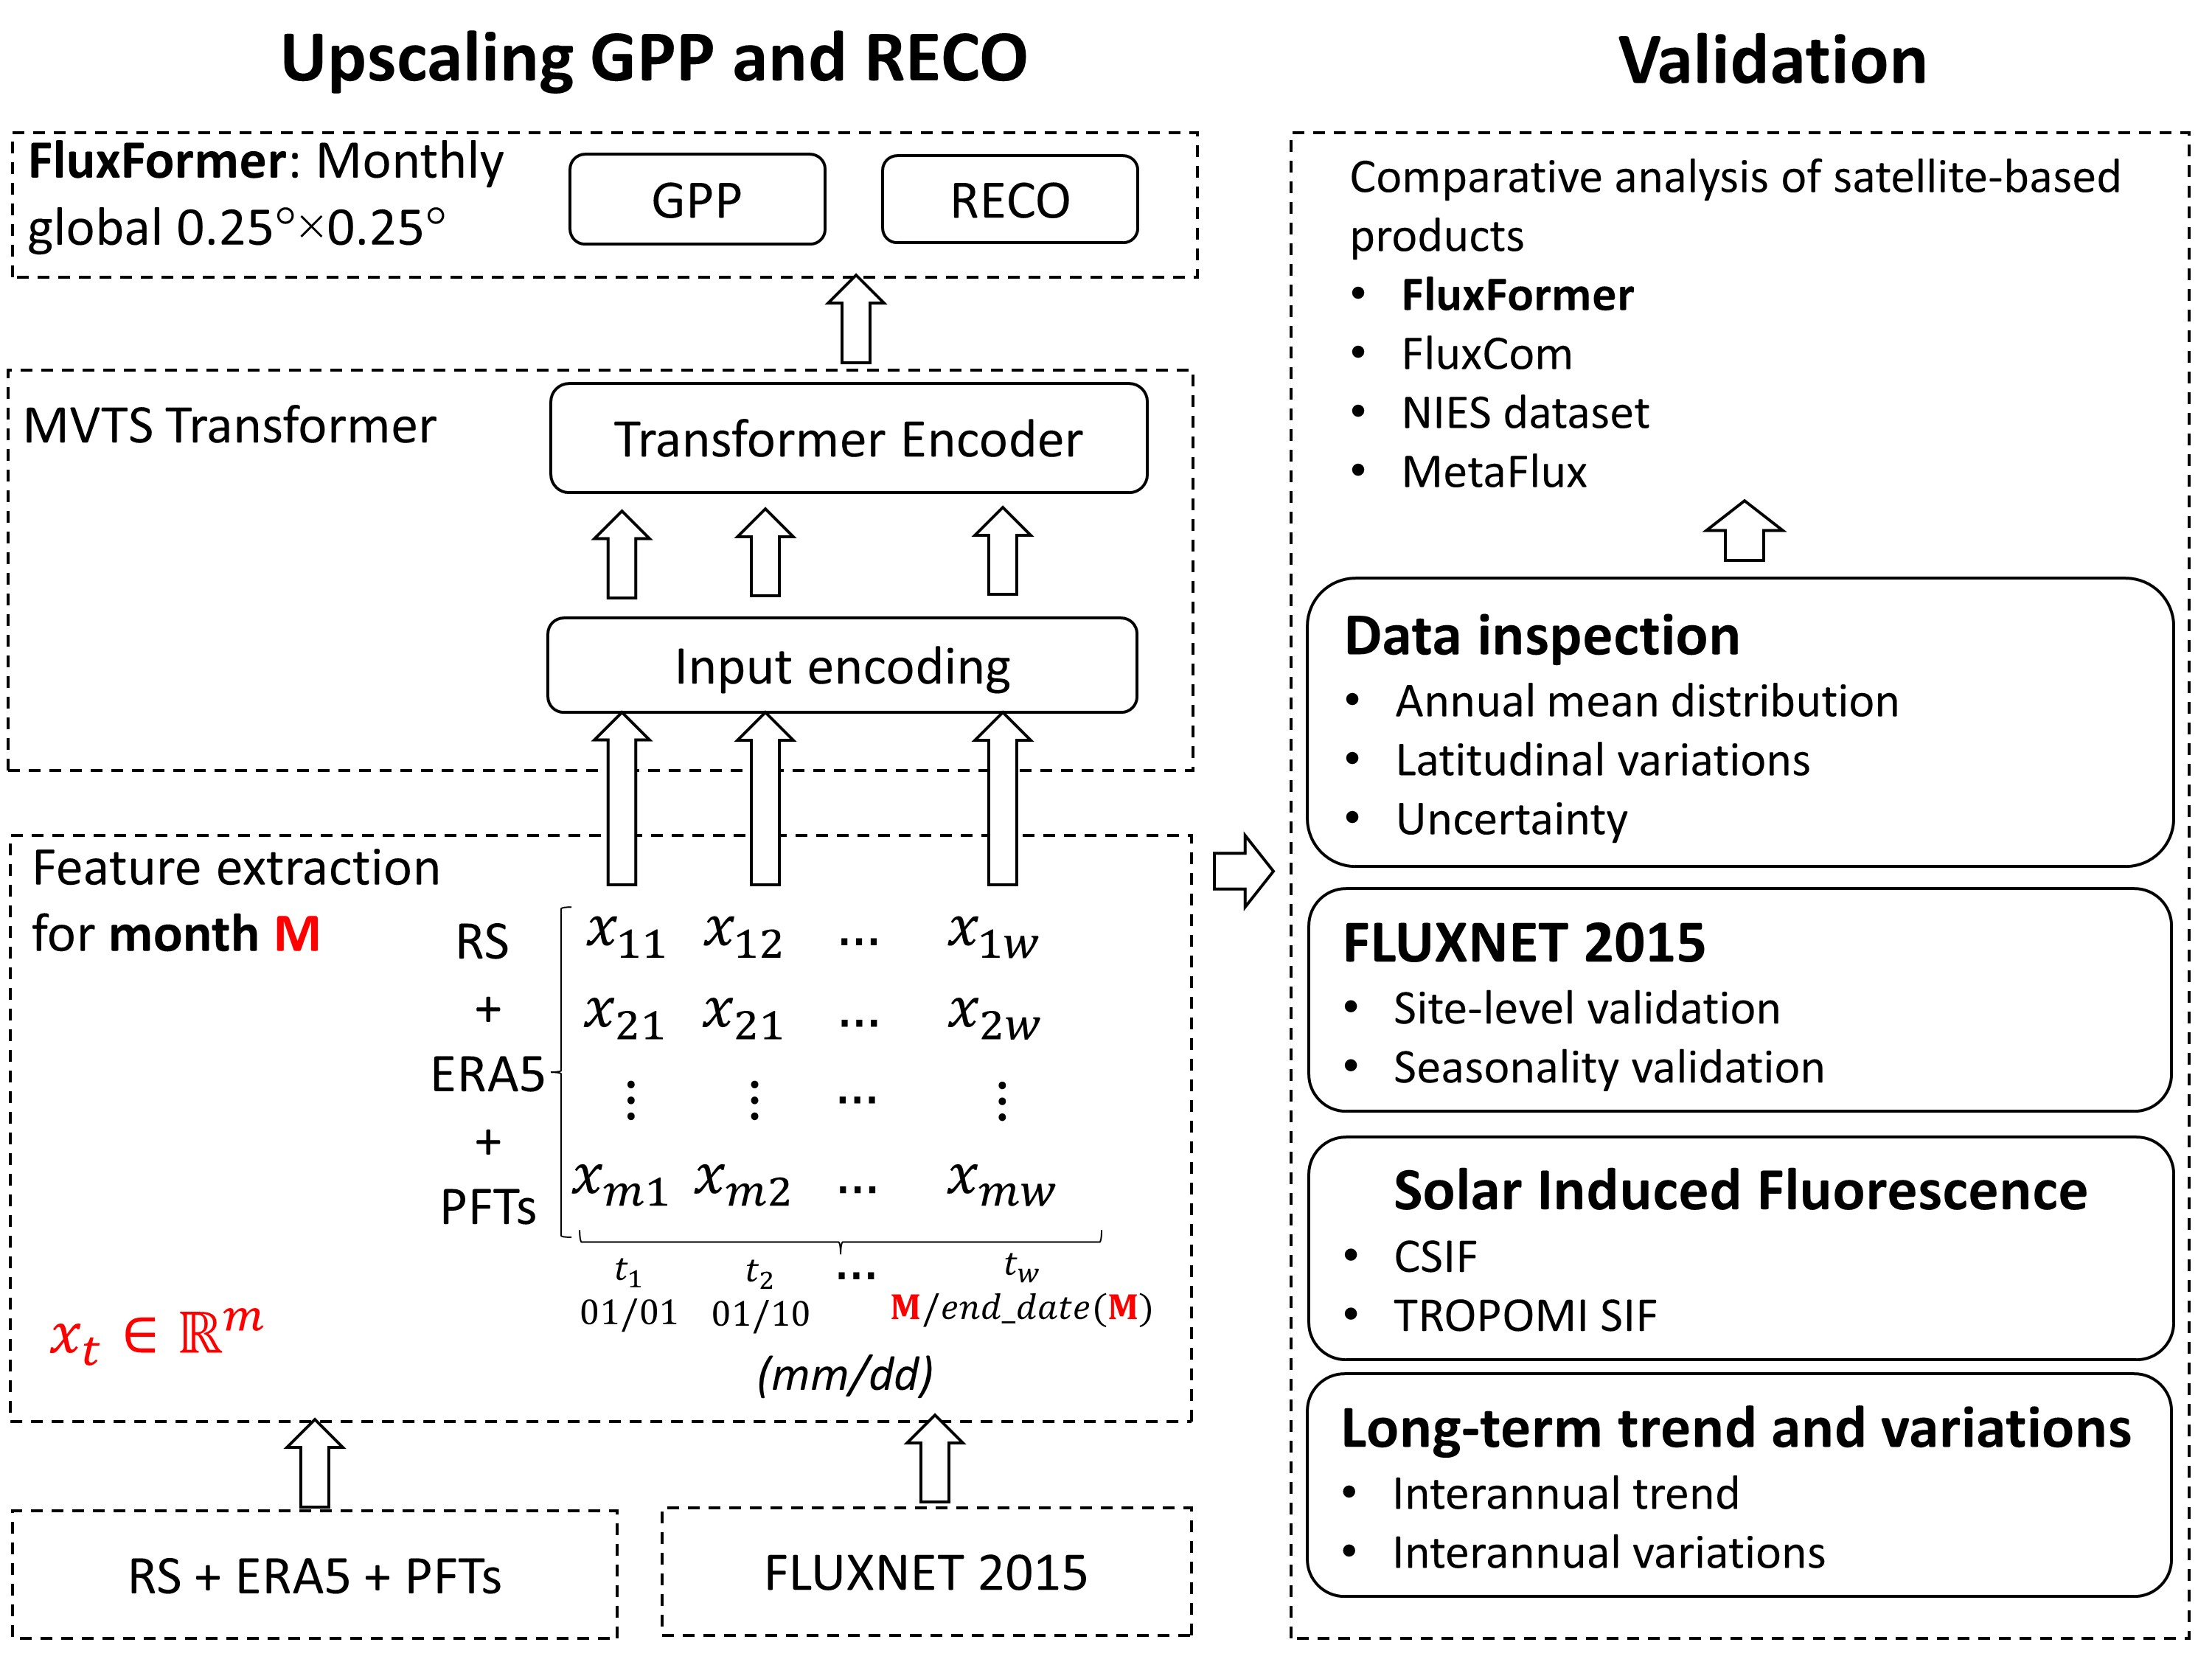
\includegraphics[width=\textwidth]{figs/chap6/workflow.jpg}
    \caption[Schemantic workflow of our FluxFormer methodology]{Schemantic workflow of our FluxFormer methodology}
    \label{fig:chap6_fig1}
\end{figure}

\subsection{Methods}
\subsubsection{Input data}

\myparagraph{FLUXNET 2015}
The FLUXNET 2015 dataset \citep{pastorello2020fluxnet2015} serves as the groundtruth for carbon fluxes in the transformer model in this study. Monthly GPP and RECO data were extracted from the dataset tier 1 of FLUXNET 2015, encompassing data from 206 sites. We filtered out records with a quality control value of less than 80\% for measured and good-quality gap-fill data. Relying solely on quality control values is reported to be insufficient for obtaining qualified data due to inconsistencies in the differences between GPP, RECO, and NEE \citep{zeng2020global, tramontana2016predicting}. Following the approach of \citep{zeng2020global}, we also excluded records with an absolute difference between GPP-RECO and NEE larger than 0.1 gC $m^{-2} d^{-1}$.
\myparagraph{Remote sensing data}
For the remote sensing data, we employed version 2 of the global leaf area index (LAI) and fraction of absorbed photosynthetically active radiation (FAPAR) datasets, generated using the algorithm proposed by \citep{verger2014near}. These datasets can be accessed through the Copernicus Global Land Service, providing a 1 km spatial resolution for every 10 days spanning from 1999 to 2019. The remote sensing data utilized in this study is in line with the approach presented in \citep{zeng2020global}. The latitude boundary of this dataset ranges from -60°S to 80°N. \par
\myparagraph{Meteorological data}
For meteorological data, we employed specific variables from the ERA5 reanalysis product \citep{hersbach2020era5}, including 2-meter air temperature (T2M), surface short-wave (solar) radiation downwards (SSRD), vapor pressure deficit (VPD), total precipitation (TP), and evaporation (E). As VPD is not directly available in the original dataset, we estimated it using the relationship between saturated vapor pressure (SVP) and actual vapor pressure (AVP): VPD = SVP - AVP, based on 2-meter air and dewpoint temperature. The original spatial resolution of ERA5 data is 0.25° × 0.25° and was obtained from the Copernicus Climate Change Service (C3S) Climate Data Store (CDS). \par

\myparagraph{Plant function types}
The PFTs dataset employed in this study, denoted as PFT v2.0.8 and obtained from \citep{harper202229}, spans the period from 1992 to 2020. It provides the specific percentage cover of 14 PFTs for each pixel at a 300m resolution. The annual dataset comprises 14 layers, with pixel values at 300m resolution indicating the percentage cover (ranging from 0\% to 100\%) for each of the 14 PFTs. This updated PFTs dataset is considered a more accurate representation of PFT distributions as it relies on high-resolution, peer-reviewed mapping of specific vegetation classes to refine global assumptions about PFT fractions \citep{harper202229}. Regional updates in PFT fractions are anticipated to enhance carbon fluxes estimation. The complete set of PFTs includes bare soil, built areas, water bodies, snow and ice, natural grasses, managed grasses (i.e., herbaceous cropland), broadleaved deciduous trees, broadleaved evergreen trees, needleleaved deciduous trees, needleleaved evergreen trees, broadleaved deciduous shrubs, broadleaved evergreen shrubs, needleleaved deciduous shrubs, and needleleaved evergreen shrubs. The dataset can be accessed from the CEDA archive at https://catalogue.ceda.ac.uk/uuid/26a0f46c95ee4c29b5c650b129aab788.\par

\subsubsection{Multivariate Time Series Transformer Framework}
Figure \ref{fig:chap6_fig1} illustrates the overall workflow of our FluxFormer methodology to upscale GPP and RECO from remote sensing data, and PFTs data. We utlized the original Multivariate Time Series MVTS Transformer model which is transformer-based framework proposed by \citep{zerveas2021transformer} which contains an input encoding layer with learnable positional encoding and a Transformer Encoder \citep{vaswani2017attention}. MVTS Transformer achieved good performance on supervised and unsupervised regression task based on multivariate time series representation even with limited training samples.  \par
In order to train the MVTS Transformer, first, we extracted the remote sensing data, meteorological data and PFTs for each monthly record from FLUXNET 2015 dataset. Then the extracted data is formed to feed to the deep learning model. In particular, for a specific month \textbf{M}, each traing sample $\mathbf{X} \in \mathbb{R}^{w\times n}$ where \textit{w} is the lengths of timeseries for month \textbf{M} ($\textit{w} = 3\times \textbf{M}$ as we have three remote sensing products per month) and \textit{m} is the number of different variables ($\textit{m} = 21$ 2 remote sensing varibales (LAI and FAPAR), 5 meteorological variables (T2M, SSRD, VPD, TP, E) and 14 PFTs variables), constitutes a sequence of \textit{w} feature vectors $\mathbf{x}\textsubscript{t} \in \mathbb{R}^{m}: \mathbf{X} \in \mathbb{R}^{w\times n} = [\mathbf{x}\textsubscript{1},\mathbf{x}\textsubscript{1}, \dots, \mathbf{x}\textsubscript{w}]$ is a multivariate timeseries of length \textit{w} and \textit{m} different variables. \par

\subsubsection{Training setup}
To train the model, approximately 80\% of the monthly data was randomly chosen for training, while the remaining 20\% was allocated for validation. Twelve models were trained over the course of 12 months. \par
\begin{table}[!ht]
    \centering
    \caption{Number of samples for training and validation}
    \begin{tabular}{ccc}
        \hline
        \multirow{2}{*}{Month} & \multicolumn{2}{c}{Number of samples} \\ \cline{2-3}
        ~ & Training & Validation \\ \hline
        January & 295 & 68 \\ 
        February & 305 & 72 \\ 
        March & 315 & 77 \\ 
        April & 310 & 75 \\ 
        May & 320 & 88 \\ 
        June & 306 & 66 \\ 
        July & 313 & 66 \\ 
        August & 298 & 67 \\ 
        September & 319 & 68 \\ 
        October & 335 & 71 \\ 
        November & 310 & 75 \\ 
        December & 295 & 62 \\ \hline
    \end{tabular}
    \label{tab:chap6_nosamples}
\end{table}

Notably, the distribution of FLUXNET 2015 sites is uneven across climate zones, particularly in the tropics and semi-arid regions, despite the highest GPP values being observed in tropical areas such as Amazonia, Central Africa, and Southeast Asia \citep{chen2017regional}. Additionally, semi-arid regions play a crucial role in influencing the global carbon cycle \citep{poulter2014contribution}. To reduce this imbalance, we exclusively utilized the most recent data from the past three years for each site as suggested by \citep{zeng2020global}. This choice aimed to guarantee a fairer representation of each site during the training of the transformer model. This approach yielded a total of 4576 samples over the 12-month period, derived from the pool of 10655 qualified monthly samples. The distribution of samples for training and validation is outlined in Table \ref{tab:chap6_nosamples}. \par
\subsubsection{Validation}
FluxFormer's quality was assessed through comprehensive comparisons. First, we examined the annual mean distribution as well as latitudinal variations of FluxFormer and other products. To evaluate uncertainties in our analysis, we employed bootstrapping. We generated 100 separate samples of the eddy covariance data, ensuring each sample contained a balanced representation of different PFTs through stratification. We then trained 100 model versions on these samples and used them to make predictions. The standard deviation of these predictions represents the associated uncertainty. \par

Subsequently, we analyzed site-level correlations, errors, and seasonal patterns across climate zones by comparing monthly GPP and RECO from FLUXNET 2015 with corresponding data from leading satellite-based upscaled products like FluxCom \citep{jung2019fluxcom}, NIES \citep{zeng2020global}, and MetaFlux \citep{nathaniel2023metaflux}. \par

Next, we evaluated GPP seasonality against SIF due to its increasing use in GPP estimation \citep{norton2019estimating, liu2020improving, bai2022estimation}. We incorporated independent products, namely CSIF \citep{zhang2018global}, and TROPOMI SIF \citep{kohler2018global}. We examined the pixel-level correlation distribution of FluxFormer and selected satellite-based products with the seasonal trend of CSIF from 2000 to 2019 and TROPOMI SIF from 2018 to 2019, as TROPOMI data is available only from 2018 onwards. \par

Finally, we examined the interannual trends and variations of our data FluxFormer in comparison with FluxCom, NIES, and MetaFlux. To evaluate interannual trends, we computed the annual global mean GPP and RECO, scaling the global average fluxes using the total global land area of 122.4 million square kilometers \citep{friedl2010modis}, as recommended by \citep{jung2020scaling} to ensure consistent global area representation across all products. The annual trends and their statistical significance in GPP and RECO were indicated by the slope of the linear regression line and the corresponding p-value. For the assessment of interannual variations, we determined the Interannual Variability (IAV) at the pixel level by calculating the standard deviation divided by the mean of annual fluxes.\par

\subsection{Data records}
We provided global monthly data of GPP and RECO available at 0.25-degree spatial resolution from 1999 to 2019. The latitude boundary extends from -60°S to 80°N which is same as the latitude boundary of the remote sensing used in this study. The longitude extends from -180°W to 180°S. The data is provided in Network Common Data Form (NetCDF) format. The data variables are defined by time, latitude, longitude coordinates. In the provided data, we purposely masked out the cold regions that consist of the Arctic circle and the desert region. The FluxFormer GPP and RECO products are available at \url{https://doi.org/10.5281/zenodo.10258644}.\par

\begin{figure}[tbh!]
    \centering
    \includegraphics[width=\textwidth]{figs/chap6/mean_GPP_RECO.jpg}
    \caption[Mean estimate of GPP and RECO in 2017]{Mean estimate of (a) GPP and (b) RECO for the year 2017: GPP (a) RECO (b)}
    \label{fig:chap6_fig2}
\end{figure}
\begin{figure}[h!]
  \centering
  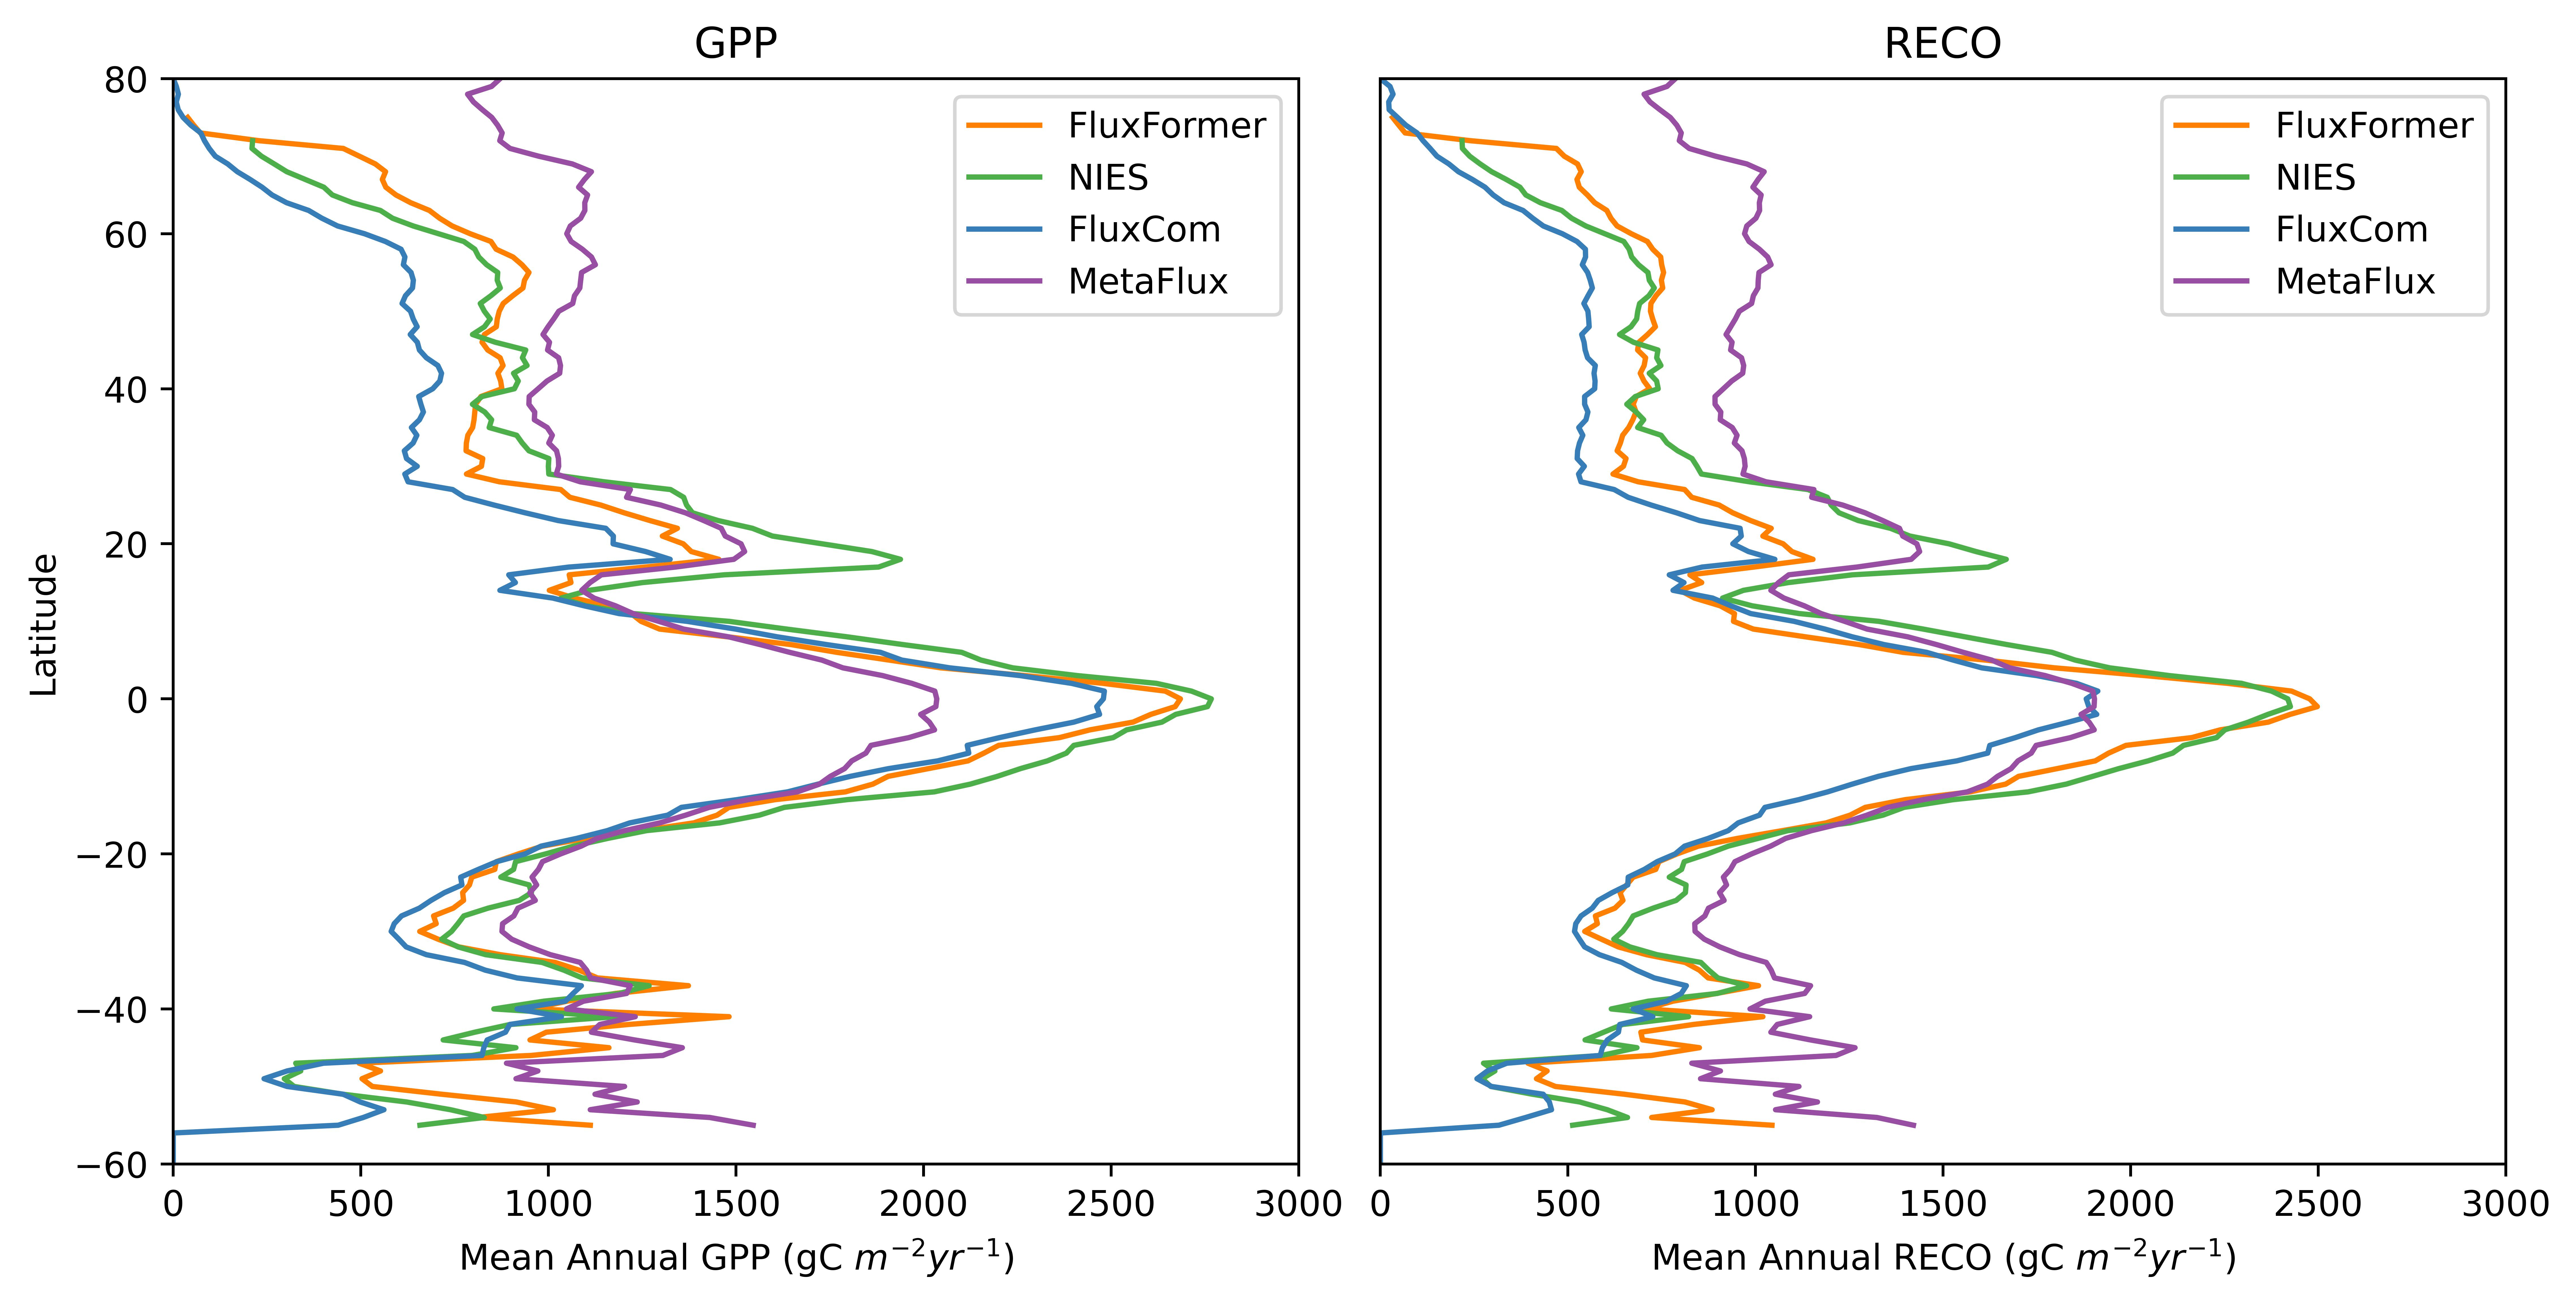
\includegraphics[width=\textwidth]{figs/chap6/lat_mean.jpg}
  \caption[Latitudinal distribution of mean annual GPP and RECO]{Latitudinal distribution of mean annual GPP and RECO from 2001 to 2019}
  \label{fig:chap6_fig_lat_mean}
\end{figure}
\begin{figure}[h!]
  \centering
  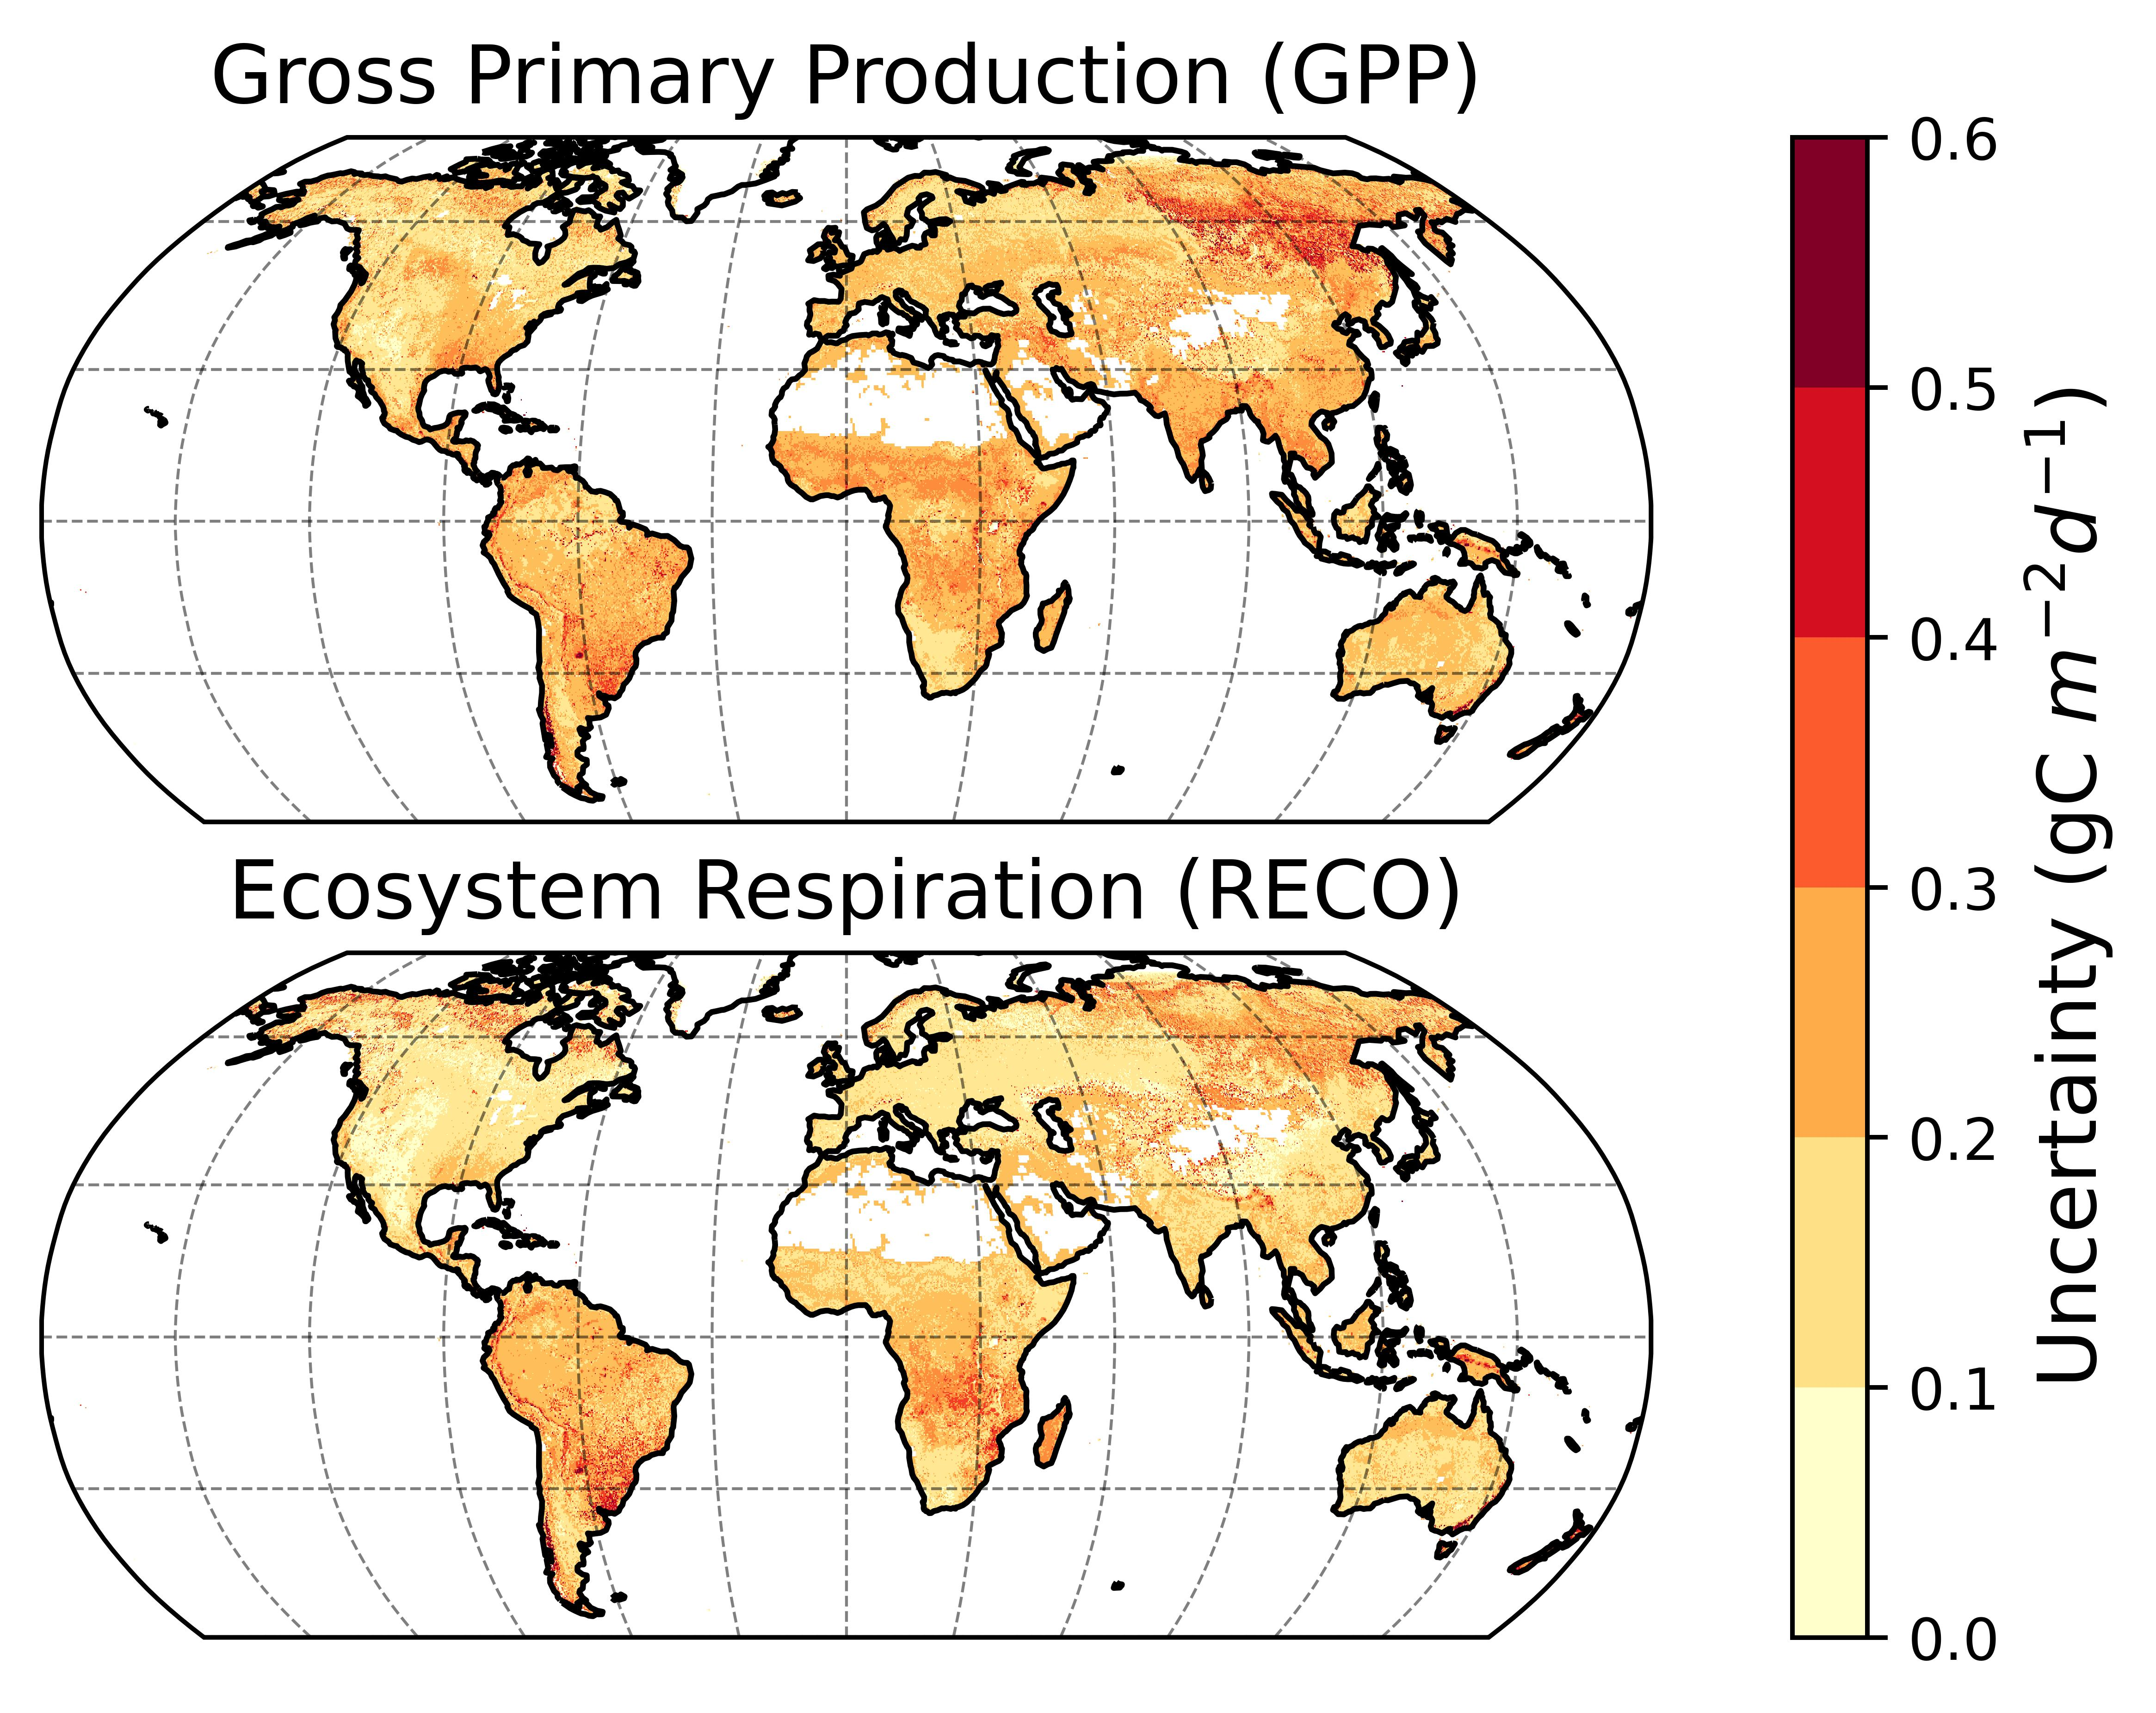
\includegraphics[width=\textwidth]{figs/chap6/uncertainty.jpg}
  \caption{Estimated uncertainty for the year 2017 of GPP and RECO}
  \label{fig:chap6_fig_std}
\end{figure}

Figure \ref{fig:chap6_fig2} illustrates the average GPP and RECO values for all products in 2017. As expected, both GPP and RECO are highest in tropical regions and lowest in semi-arid areas. Notably, the largest differences between product estimates occur in tropical regions, likely due to variations in input data and methodological approaches. Figure \ref{fig:chap6_fig_lat_mean} depicts the latitudinal distribution of GPP and RECO. A consistent pattern emerges across all products, with both GPP and RECO values gradually increasing from colder climates towards warm and humid conditions in temperate and tropical regions. Figure \ref{fig:chap6_fig_std} illustrates the uncertainty in predicted carbon fluxes for an example year (2017) through the standard deviation of predictions from 100 bootstrapped models. As expected, tropical regions exhibit notably higher uncertainty. This likely reflects the scarcity and uneven distribution of EC measurement sites in these areas, limiting the data available for model training and validation. \par

\subsection{Technical validation}
\subsubsection{Validation with FLUXNET 2015}
\myparagraph{Site-level validation}
We utilized the Pearson Correlation Coefficient (R) and Root Mean Square Error (RMSE) to assess the quality of our products in comparison to FLUXNET 2015 observations. As depicted in Figures \ref{fig:chap6_fig3a} and \ref{fig:chap6_fig3b}, our product demonstrates the highest correlation and the lowest RMSE with FLUXNET 2015 for both GPP and RECO data ($r = 0.89, RMSE = 1.74$ for GPP and $r = 0.86, RMSE = 1.26$ for RECO). In contrast, MetaFlux shows the lowest correlation with FLUXNET 2015 ($r = 0.6, RMSE = 3.16$ for GPP and $r = 0.56, RMSE = 2.08$ for RECO). NIES and FLUXCOM also exhibit strong correlations with the ground truth data, achieving $r/RMSE: 0.88/1.78$ (NIES), $0.81/2.31$ (FLUXCOM) for GPP and $r/RMSE: 0.84/1.35$ (NIES), $0.79/1.64$ (FLUXCOM) for RECO. \par

\begin{figure}[p]
    \centering
    \begin{subfigure}{\textwidth}
      \centering
      \includegraphics[width=.8\textwidth]{figs/chap6/val_fluxnet_all_GPP.jpg}
      \caption{GPP}
      \label{fig:chap6_fig3a}
    \end{subfigure}

    \begin{subfigure}{\textwidth}
      \centering
      \includegraphics[width=.8\textwidth]{figs/chap6/val_fluxnet_all_RECO.jpg}
      \caption{RECO}
      \label{fig:chap6_fig3b}
    \end{subfigure}
    \caption[Validation with FLUXNET 2015]{Validation with FLUXNET 2015: GPP (a) RECO (b)}
    \label{fig:chap6_fig3}
\end{figure}
\myparagraph{Seasonality validation}
We analyzed the seasonal trend using FLUXNET 2015 data, calculating monthly mean values across climate zones, as depicted in Figure \ref{fig:chap6_fig4} and Table \ref{tab:chap6_seasonr}. In arid regions, FluxFormer, FluxCom, and NIES exhibited high correlation ($r > 0.9$) with FLUXNET for both GPP and RECO. However, MetaFlux showed lower correlation with $r=0.48$ for GPP and $r=0.66$ for RECO in arid regions. For temperate and cold regions, all satellite-based products (FluxFormer, FLUXCOM, NIES, and MetaFlux) demonstrated high correlations ($r>0.9$) with FLUXNET 2015 GPP and RECO. \par

\begin{table}[!ht]
    \centering
    \caption{Pearson correlation of seasonal trend with FLUXNET 2015}
    \begin{tabular}{ccccc}
        \hline
        Climate groups & FluxFormer & FluxCom & NIES & MetaFlux  \\ \hline
        \multicolumn{5}{c}{GPP}   \\ \hline 
        Arid & 0.91 & 0.90 & 0.95 & 0.48  \\ \hline 
        Temperate & 0.99 & 0.99 & 0.99 & 0.97  \\ \hline 
        Continental & 1 & 0.99 & 1 & 0.99  \\ \hline 
        Trop. SVN & 0.99 & 0.99 & 0.96 & 0.98  \\ \hline 
        Trop. MS & \textbf{0.84} & 0.04 & 0.78 & -0.1  \\ \hline 
        Trop. RF & 0.68 & 0.6 & 0.8 & 0.42  \\ \hline 
        \multicolumn{5}{c}{RECO}   \\ \hline 
        Arid & 0.94 & 0.92 & 0.96 & 0.66  \\ \hline 
        Temperate & 0.98 & 0.99 & 0.99 & 0.99  \\ \hline 
        Continental & 1 & 0.99 & 1 & 1  \\ \hline 
        Trop. SVN & 0.99 & 0.98 & 0.94 & 0.92  \\ \hline 
        Trop. MS & \textbf{0.88} & 0.51 & 0.21 & 0  \\ \hline 
        Trop. RF & \textbf{0.68} & 0.37 & 0.49 & 0.47  \\ \hline 
    \end{tabular}
    \label{tab:chap6_seasonr}
\end{table}
\begin{figure}[p]
    \centering
    \begin{subfigure}{\textwidth}
      \centering
      \includegraphics[width=.8\textwidth]{figs/chap6/seasonal_fluxnet_GPP.jpg}
      \caption{GPP}
      \label{fig:chap6_fig4a}
    \end{subfigure}

    \begin{subfigure}{\textwidth}
      \centering
      \includegraphics[width=.8\textwidth]{figs/chap6/seasonal_fluxnet_RECO.jpg}
      \caption{RECO}
      \label{fig:chap6_fig4b}
    \end{subfigure}
    \caption[Seasonality validation with FLUXNET 2015]{Seasonality validation with FLUXNET 2015: GPP (a) RECO (b)}
    \label{fig:chap6_fig4}
\end{figure}
In the tropical region, we partitioned the area into tropical savanna (Trop. SVN), tropical monsoon (Trop. MS), and tropical rainforest (Trop. RF). In Trop. SVN, all satellite-based products displayed a high correlation with FLUXNET 2015 for both GPP and RECO. Conversely, for Trop. MS, our data exhibited the highest correlation at $r=0.84$, while NIES data showed a slightly lower correlation ($r=0.78$). FLUXCOM and MetaFlux demonstrated no correlation with FLUXNET 2015 for GPP, with $r<0.1$. Regarding RECO in Trop. MS, our data maintained the highest correlation with the seasonal trend of the ground truth, whereas other products showed lower correlation (FLUXCOM: $r=0.51$, NIES: $r=0.21$) or no correlation with the ground truth (MetaFlux: $r=0$). In the Trop. RF area, our data exhibited the second-highest correlation with GPP seasonal trend ($r=0.68$) and the highest correlation with RECO seasonal trend ($r=0.68$).\par
Overall, our data demonstrates a robust correlation in arid, temperate, continental, and Trop. SVN regions, surpassing $r> 0.9$ for both GPP and RECO. Specifically, in Trop. MS, our data exhibits the highest correlation, reaching $r=0.84$ for GPP and $r=0.88$ for RECO. In the Trop. RF region, our data exhibits the second-highest correlation with the ground truth GPP seasonal trend ($r=0.68$) and the highest correlation with the ground truth RECO seasonal trend ($r=0.68$) among the selected satellite-based products. \par


\subsubsection{Validation with SIF}
While a linear relationship between GPP and SIF has been widely assumed in previous studies \citep{guanter2012retrieval, yang2017chlorophyll}, this assumption remains uncertain across diverse climate regions and PFTs \citep{gu2019sun, xiao2019solar, zhang2016model, chen2021seasonal}. This uncertainty is particularly pronounced in tropical regions, where weak seasonality in photosynthesis leads to a less robust linear relationship between SIF and GPP \citep{doughty2021global}. Regionally, tropical forests and savannahs are often water-limited rather than sunlight-limited \citep{guan2015photosynthetic, rs9060530, Madani_2020, palmer2023drivers}. Furthermore, tropical forests, dominated by evergreen broadleaf forests (EBFs), exhibit complex vegetation structures that contribute to larger uncertainties in both satellite observations and ground-based GPP estimates from eddy covariance (EC) sites, further weakening the SIF-GPP correlation in these regions \citep{hayek201890, xietal2018, zhang2020111722, shekhar2022113282}. Additionally, frequent cloud cover in the tropics contaminates SIF signals from satellite observations, adding to the challenge of using SIF as a reliable proxy for GPP \citep{doughty2021global, shekhar2022113282}.\par

\begin{figure}[tbh!]
    \centering
    \includegraphics[width=\textwidth]{figs/chap6/val_SIF.jpg}
    \caption[Validation with SIF products]{Validation with SIF products: CSIF (a) TROPOMI SIF (b)}
    \label{fig:chap6_fig5}
\end{figure}

Figure \ref{fig:chap6_fig5} depicts the temporal correlations between monthly SIF and GPP. In temperate and continental regions, most products show moderate to high GPP-SIF correlations. CSIF (Figure \ref{fig:chap6_fig5}a) exhibits slightly higher correlations than TROPOMI SIF (Figure \ref{fig:chap6_fig5}b), likely due to its longer observation period. However, in arid regions, FluxFormer show lower GPP-SIF correlations, especially in the Horn of Africa deserts. This corresponds with the findings of \citep{palmer2023drivers}, highlighting the more substantial influence of rainfall on GPP than sunlight in this eastern desert region of Africa. In tropical regions, our data shows lower correlations with CSIF and TROPOMI SIF compared to FluxCom, NIES, and MetaFlux, particularly in Central/South America, West/Central Africa, and Southeast Asia and arid regions compared to FluxCom, NIES, and MetaFlux. This aligns with observations from previous studies \citep{sanders2016spaceborne,doughty2021global,shekhar2022113282}, suggesting weak seasonality in tropical photosynthesis weakens the GPP-SIF correlation to background levels.


\subsubsection{Interannual variations between products}

Examining the global annual time series of GPP and RECO from 2001 to 2019 (Figure \ref{fig:chap6_fig7}), we observe diverse patterns in carbon fluxes across different products. Estimated annual mean fluxes range from 120 to 150 PgC/year for GPP (Figure \ref{fig:chap6_fig7}a) and 97 to 141 PgC/year for RECO (Figure \ref{fig:chap6_fig7}b) in FluxFormer and other products. Among these, our FluxFormer dataset exhibits the most pronounced positive GPP trend, increasing at a rate of 0.45 PgC/year. NIES follows closely with a growth rate of 0.32 PgC/year. While MetaFlux suggests a subtle upward trend, its statistical significance remains uncertain (p-value = 0.08). Conversely, FluxCom shows a slight negative trend, indicating a decrease of 0.04 PgC/year in GPP. It is worth noting that the long-term GPP trends in our data and NIES align with the anticipated increase due to the CO\textsubscript{2} fertilization effect, which could potentially enhance the land carbon sink \citep{piao2020characteristics, yang2022divergent, guo2023estimating}. \par

\begin{figure}[tbh!]
    \centering
    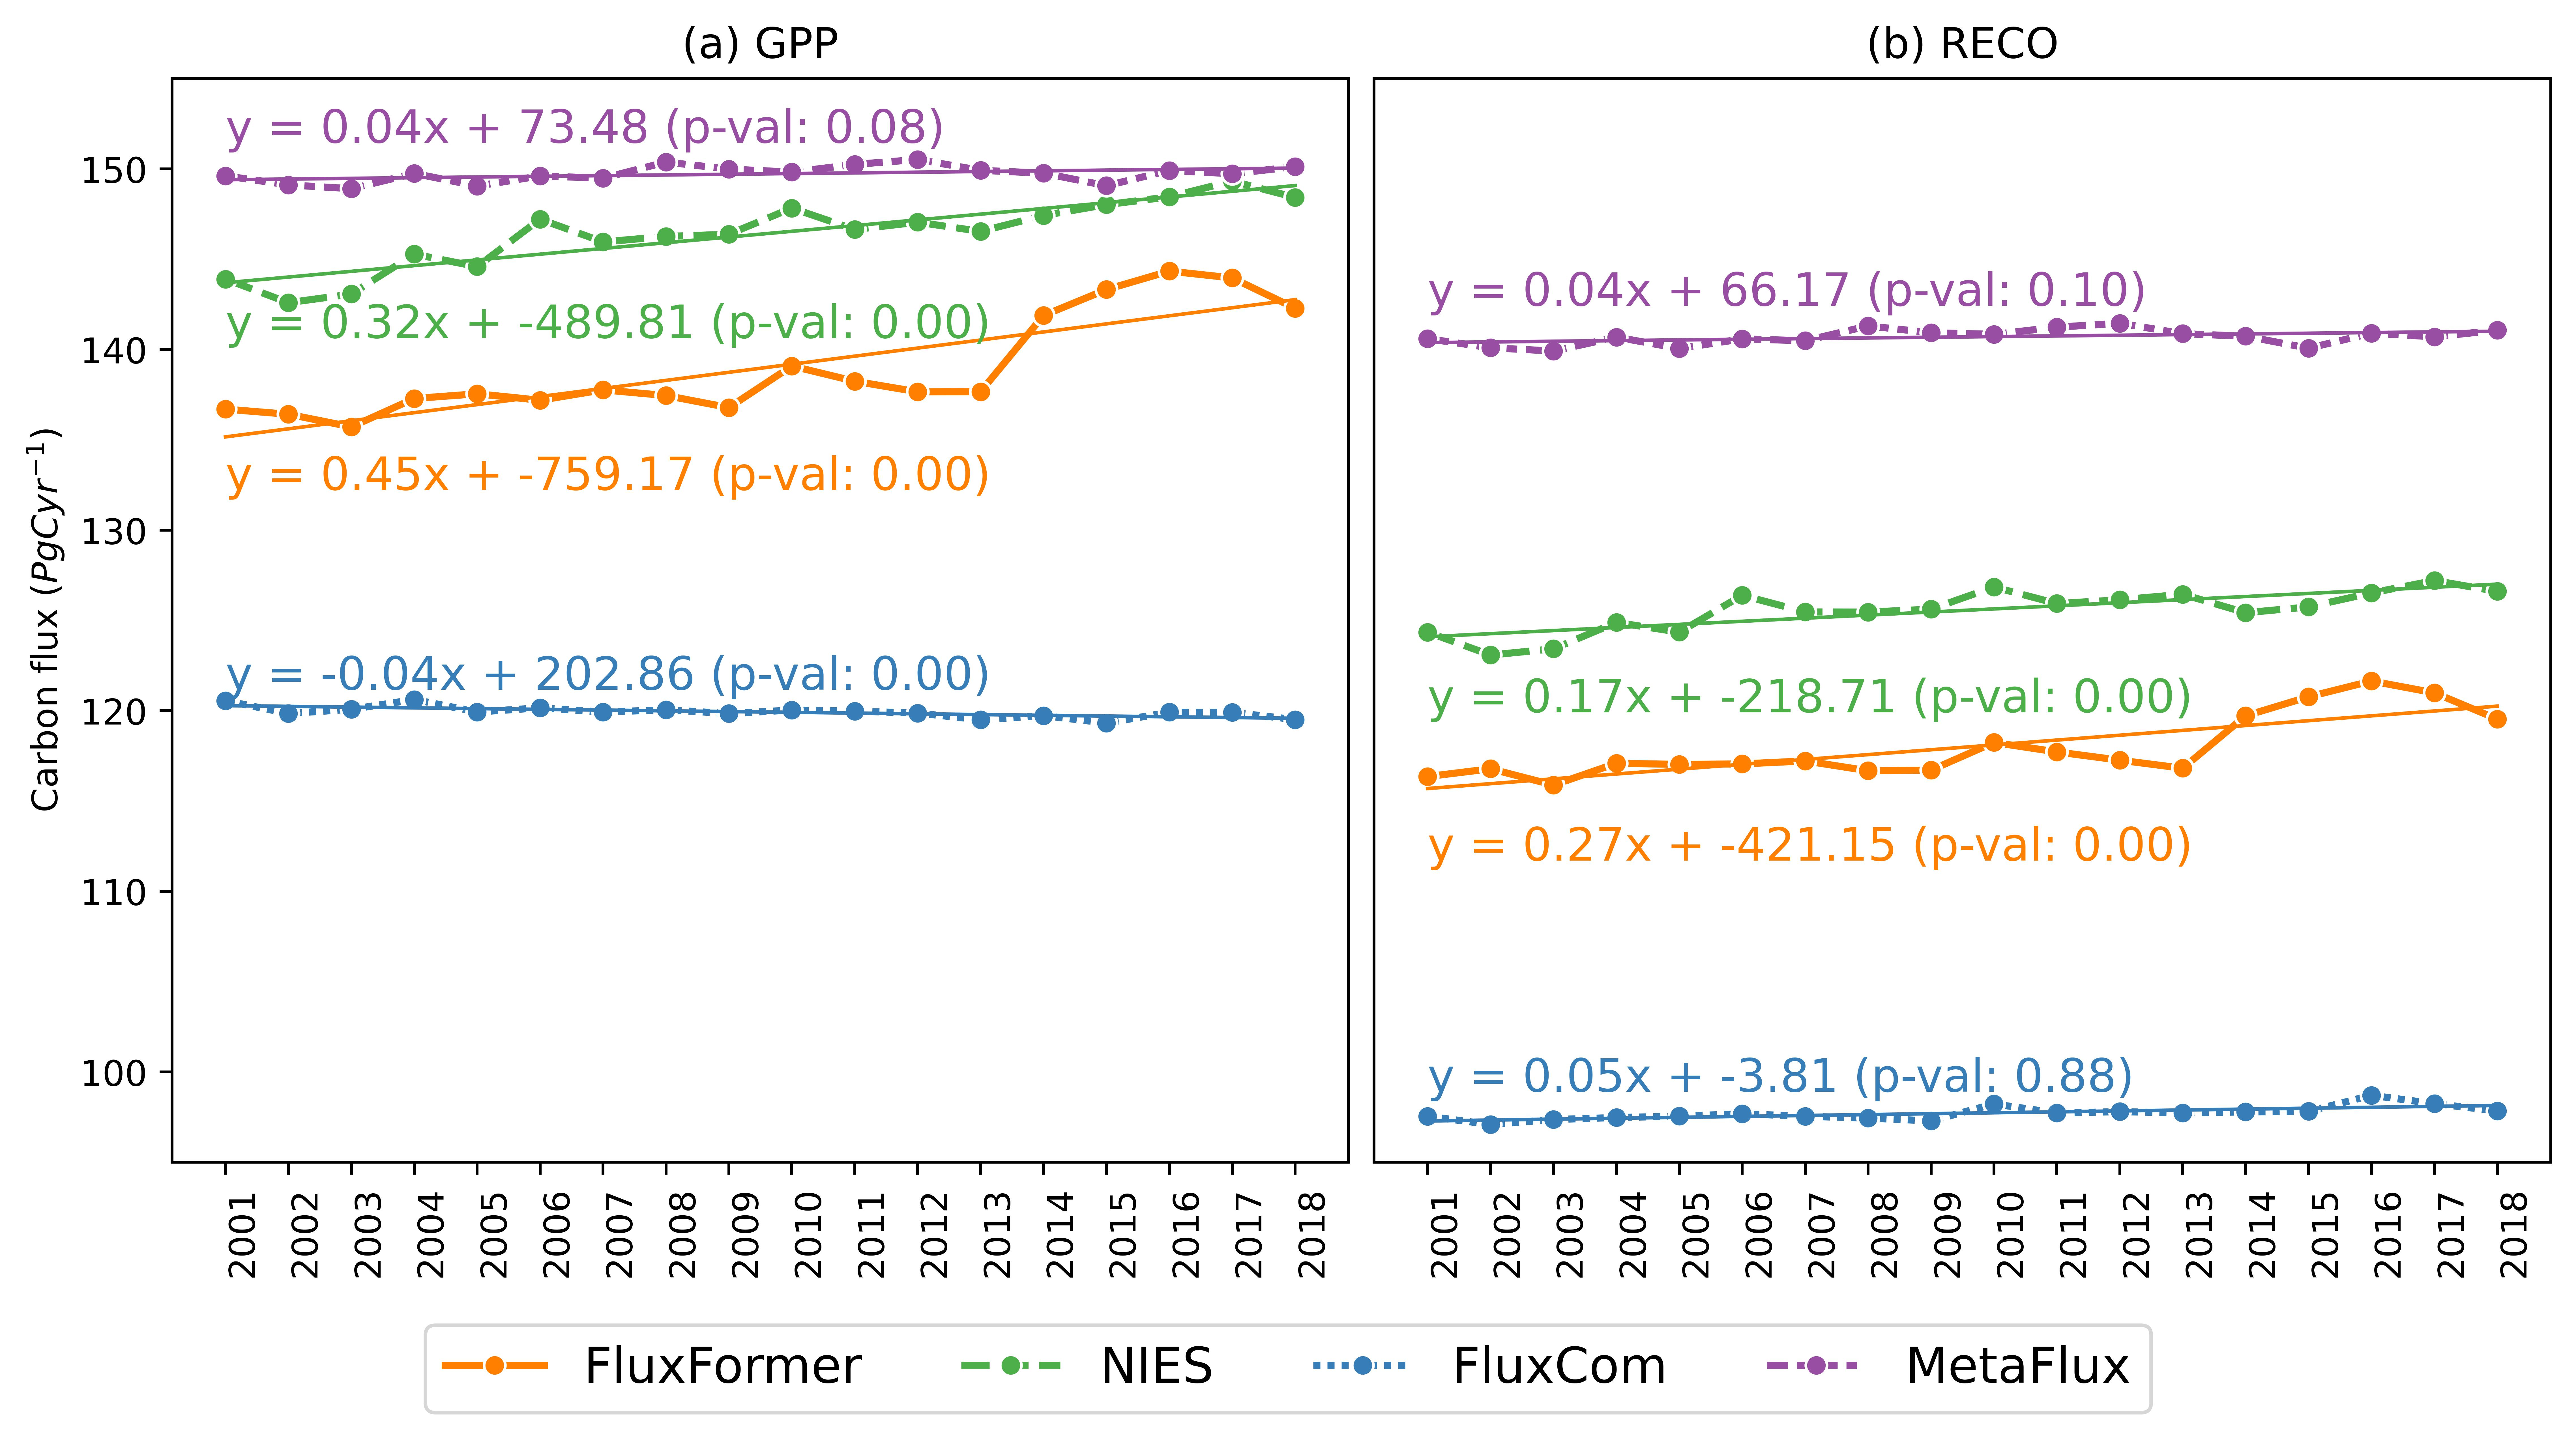
\includegraphics[width=\textwidth]{figs/chap6/global_annual_timeseries.jpg}
    \caption[Long term trend and latitudinal distribution of GPP and RECO]{Long term trend of global annual mean GPP (a) and RECO (b) from 2001 to 2019 of the four products}
    \label{fig:chap6_fig7}
\end{figure}

Focusing on interannual variations (Figure \ref{fig:chap6_fig8}), we find that our GPP data exhibits lower variability compared to NIES in desert regions like Australia, West and Central Asia, Eastern and Southern Africa, and parts of North America (Figure \ref{fig:chap6_fig8}a). This aligns with the expected low GPP in these areas \citep{hadley1981productivity}, suggesting greater plausibility of our data in these regions. However, FluxFormer displays higher interannual variability compared to FluxCom and MetaFlux. This discrepancy can be attributed to the different remote sensing data sources used for upscaling carbon fluxes. We utilize same LAI and FAPAR from SPOT/VEGETATION and PROBA-V, similar to NIES \citep{zeng2020global}. In contrast, FluxCom and MetaFlux rely on MODIS data \citep{jung2019fluxcom, nathaniel2023metaflux}. Understanding these data source differences and their potential impact on interannual variability is crucial for interpreting and comparing carbon flux estimates.\par

\begin{figure}[tbh!]
    \centering
    \includegraphics[width=\textwidth]{figs/chap6/IAV.jpg}
    \caption[Interannual variations from 2001 to 2019 of GPP and RECO]{Interannual variations from 2001 to 2019 of GPP (a), and RECO (b)}
    \label{fig:chap6_fig8}
\end{figure}
\subsection{Conclusion}
In this study, we present our work in upscaling global gross primary production and ecosystem respiration. This is achieved through the application of an MVTS Transformer model \citep{zerveas2021transformer} in conjunction with the updated global PFT data \citep{harper202229}. We provide monthly global data for GPP and RECO at a spatial resolution of 0.25° × 0.25°, covering the period from 1999 to 2019. \par

Our data show improvement with increased correlation and reduced error when compared to FLUXNET 2015 data at both the site level and seasonal trends. Notably, our data mostly exhibits strong correlations with the seasonal trends of GPP and RECO in tropical monsoon and rainforest regions. \par

We further assess the seasonal trend of our dataset using two SIF products, CSIF and TROPOMI SIF. Our dataset exhibits a strong GPP-SIF correlation in continental and temperate regions, consistent with other products. However, in tropical and semi-arid regions, our dataset shows lower GPP-SIF correlations compared to others, aligning with findings in \citep{sanders2016spaceborne,doughty2021global,shekhar2022113282}. This lower correlation is attributed to the weak seasonality in tropical photosynthesis \citep{montgomery2001forest}, making the linear GPP-SIF relationship less evident. \par

We also investigated the long-term trends of GPP and RECO from 2001 to 2019 and observed that our data exhibits the highest positive trend in GPP during this period, with a growth rate of 0.45 PgC per year. This finding aligns with previous studies \citep{piao2020characteristics, yang2022divergent, guo2023estimating}, supporting the assumption that the CO\textsubscript{2} fertilization effect should increase GPP over time. In contrast, MetaFlux and FluxCom fail to replicate the long-term trend of GPP, contradicting the currently recognized significant greening observed from regional to global scales \citep{piao2020characteristics}. \par

Lastly, we examined the interannual variations of FluxFormer in comparison with other datasets. We observed that FluxFormer exhibits lower variations in extreme-low-GPP regions, such as deserts and semi-arid regions, when utilizing the same source of remote sensing data as NIES. However, FluxFormer shows higher variations than FluxCom and MetaFlux, possibly due to the utilization of different remote sensing resources. \par